% meta.concepts: 2D moment equilibrium
% meta.tags: realistic
% acknowledge: Engineering Statics: Open and Interactive
% source: Exercise 4.9 of online edition

An L-shaped bracket is supported by a frictionless pin at $A$ and a cable between points $B$ and $D$.  Determine the tension in the cable required for equilibrium when a $70 N$ force $\bar{F}$ is applied to the bracket as shown at point $C$. 


\textit{Tip: Since the object is in equilibrium $\sum M_A = 0$ implies that the opposing moments must have equal magnitudes.}

\begin{figure}[ht!]
  \centering
  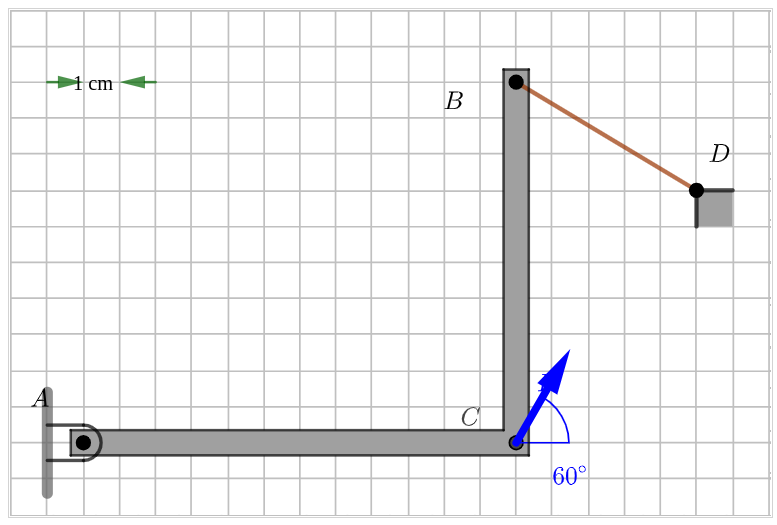
\includegraphics[width=0.5\textwidth,height=0.5\textheight,keepaspectratio]{fig.png}
\end{figure}

\iftoggle{flagSoln}{%
\vspace{.5cm}
\rule{\textwidth}{.4pt}
\vspace{.5cm}
\textbf{Solution:}
\begin{enumerate}
  \item $M_F = 727.5 N \cdot cm$
  \item $T = 49.32 N$
\end{enumerate}
\begin{figure}[ht!]
  \centering
  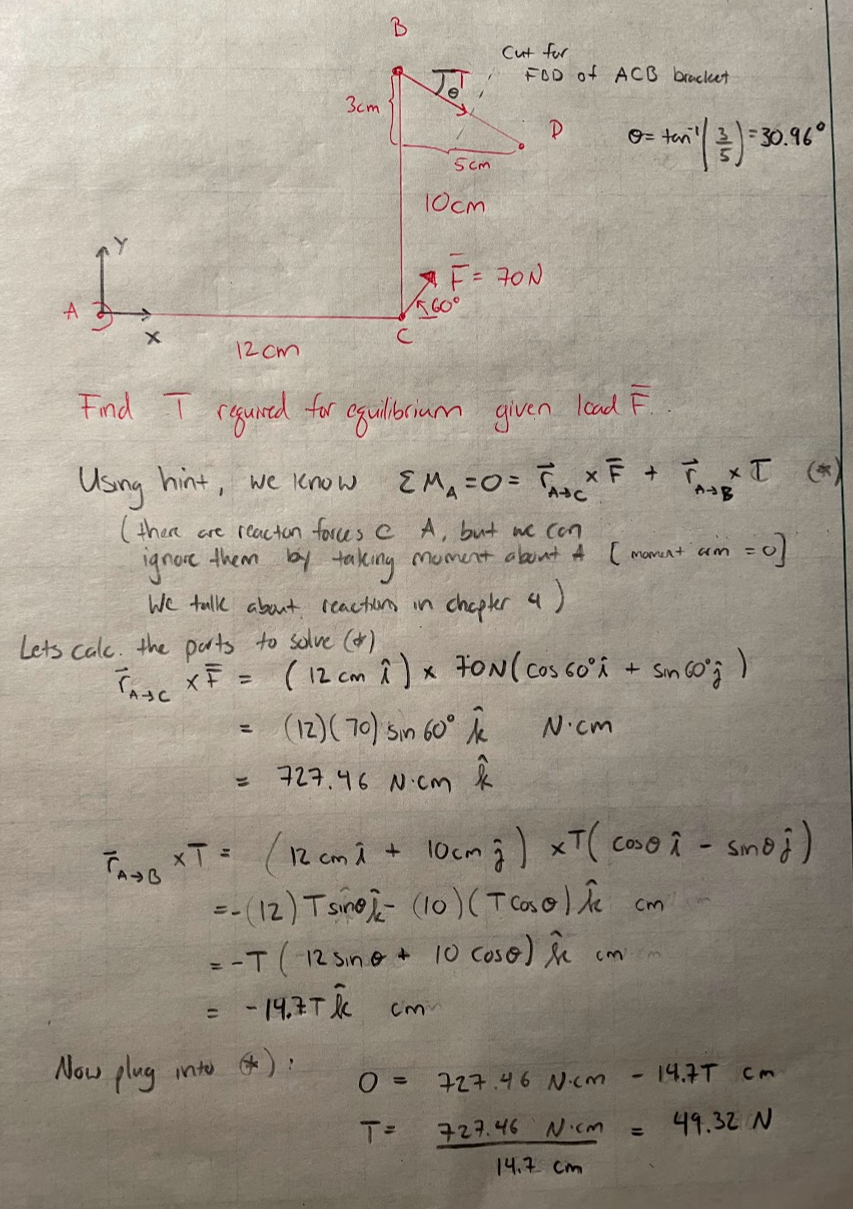
\includegraphics[width=0.9\textwidth,
	           height=0.4\textheight,
		   keepaspectratio]{soln.png}
\end{figure}

}{%
}%

